
\subsection{Serial Peripheral Interface} 

by Rustam and Nikola

% To continue the conversation about SPI. Nikola and I reviewed our reference design and prepared notes and suggestions for the SPI design.
Looking at SPI slave digital core I see that it will be impossible to redesign it manually to 3.3V. First of all, it will be mess for our layout engineers, because there are too many unstructured cells in this design. PnR is going to be a very exhausting job.

As for the register bank, I suppose that we can do it manually due to repetitive structure it will be copy/paste as Guenter mentioned before.
I prepared a block diagram with my design suggestions. In this example I'm using byte addressing according to existing memory allocation.
 
Here I'm assuming IO cells with 3.3V coreside. So, we should put level shifters from 3.3V to 1.2V on SPI ports. If we will have IO cells with 1.2V coreside we could drop out this level shifters group.

Then we have digital core SPI slave on core logic 1.2V that we will design using standard digital flow using genus/innovus and so on. Then we should put other level shifters from 1.2V to 3.3V on register bank control signals. There won't be many of them, only 21 units. Then we have 3.3V supplied register bank.

For register bank we must get some clock to store data. I see 3 options where we can get clock: 

\begin{itemize}
	\item [1.] we can use existing clock SCLK from SPI port, this way is not ideal, but if we have few free pads, we can go this way.
	\item [2.] we can use external clock from pad, it is preferable option.
	\item [3.] we can use internal generated clock from RC generator, but we should design it at first
\end{itemize}

Talking about core supply rails I see two options: external Vdd pad or internal regulator which, as I understand it, we don't have now either. 
First option with external pad is preferable, but again we will need one more pad.

We should decide which way we choose depending on our possibilities and go on.

\begin{figure}[ht!]
	\centering
	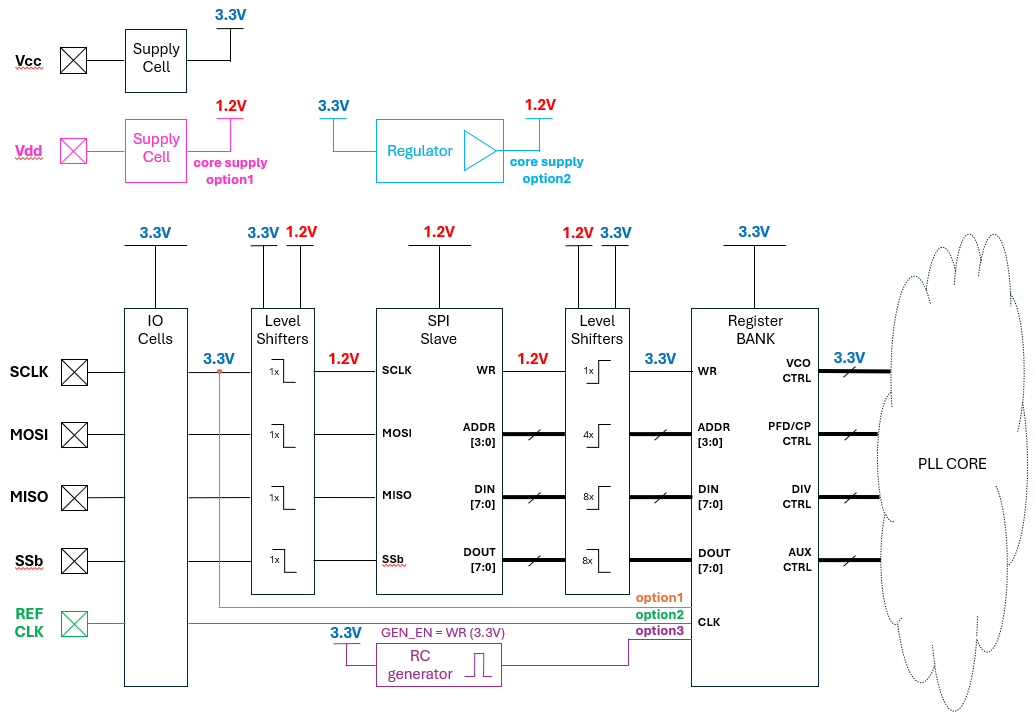
\includegraphics[width=0.5\linewidth]{Figures/spi-suggestion.png}
	\caption{SPI block scheme suggestion}
	\label{fig:spi-suggestion}
\end{figure}


% Nikola and I started working on the SPI. I have one note.
There may be some inconsistency in your proposed requirements. I would like to investigate this to make things clearer.
Your memory allocation assumes byte addressing and has 13 bytes of data. If we are talking about byte addressing, then we need 4 address bits.
But your SPI format proposes 12-bit word addressing and only 3 address bits, plus 1-bit used for R/W annotation.

Test Chip Draft Memory Allocation


\begin{figure}[ht!]
	\centering
	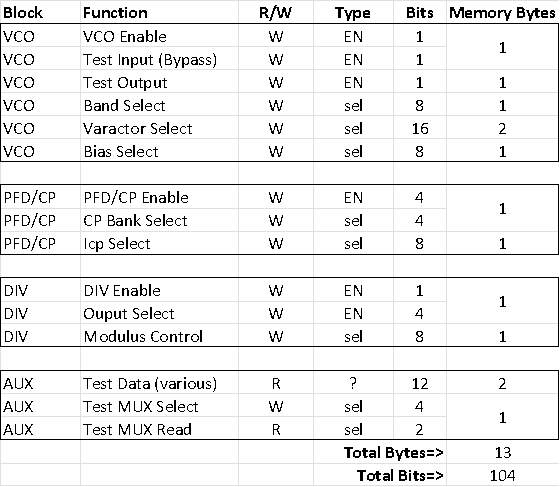
\includegraphics[width=0.5\linewidth]{Figures/test-chip-spi-draft-memory-alloc.png}
	\caption{Test Chip SPI Draft Memory Allocation}
	\label{fig:test-chip-spi-draft-memoery-alloc}
\end{figure}


Basic Format:
Total wordlength: 16bit, 
ADDR, R/W: upper 4bits,
Data: lower 12b for data 
Options:
Adding a test loop for the SPI to verify writes by reading register content back
8 or 12b readback
 
Then I see two options for resolving the issue:

Option 1:
We can use byte addressing according to existing memory allocation. So, we will use 4 address bits to allocate up to 16 bytes.
In this case we should change the command format to: 3 MSB bits - don't care; ADDR - 4 bits; R/W - LSB bit of first byte; DATA - second byte 

\begin{table}[!ht]
    \centering
    \begin{tabular}{|l|l|l|l|l|l|l|l|l|l|}
    \hline
        CMD format & CMD Byte 1 & ~ & ~ & ~ & ~ & ~ & ~ & ~ & CMD Byte 2 \\ \hline
        ~ & 7 & 6 & 5 & 4 & 3 & 2 & 1 & 0 & 7 \\ \hline
        option 1 & x & x & x & A3 & A2 & A1 & A0 & RW & D7 \\ \hline
        option 2 & A2 & A1 & A0 & RW & D11 & D10 & D9 & D8 & D7 \\ \hline
    \end{tabular}
\end{table}


Option 2:
We can use addressing according to your proposed command format. So, we will use 3 address bits to allocate up to 8 words with 12-bit word length.
In this case we should change existing memory allocation table. This is the example:



\begin{table}[!ht]
    \centering
    \begin{tabular}{|l|l|l|l|l|l|l|l|l|l|}
    \hline
        Block & Function & R/W & Type & Bits & \#Bit & \#Word  & ~ & ~ & CMD Byte 2 \\ \hline
        VCO & VCO Enable & W & EN & 1 & 0 & 0 & 1 & 0 & 7 \\ \hline
        VCO & Test Input (Bypass) & W & EN & 1 & 1 & ~ & A0 & RW & D7 \\ \hline
        VCO & Test Output & W & EN & 1 & 2 & ~ & D9 & D8 & D7 \\ \hline
        VCO & Band Select & W & sel & 8 & 3:10 & ~ & ~ & ~ & ~ \\ \hline
        ~ & Dummy & ~ & 11 & ~ & ~ & ~ & ~ & ~ & ~ \\ \hline
        ~ & ~ & ~ & ~ & ~ & ~ & ~ & ~ & ~ & ~ \\ \hline
        VCO & Varactor Select part 1 & W & sel & 12 & 0:11 & 1 & ~ & ~ & ~ \\ \hline
        ~ & ~ & ~ & ~ & ~ & ~ & ~ & ~ & ~ & ~ \\ \hline
        VCO & Varactor Select part 2 & W & sel & 4 & 0:3 & 2 & ~ & ~ & ~ \\ \hline
        VCO & Bias Select & W & sel & 8 & 4:11 & ~ & ~ & ~ & ~ \\ \hline
        ~ & ~ & ~ & ~ & ~ & ~ & ~ & ~ & ~ & ~ \\ \hline
        PFD/CP & PFD/CP Enable & W & EN & 4 & 0:3 & 3 & ~ & ~ & ~ \\ \hline
        PFD/CP & CP Bank Select & W & sel & 4 & 4:7 & ~ & ~ & ~ & ~ \\ \hline
        PFD/CP & Icp Select part 1 & W & sel & 4 & 8:11 & ~ & ~ & ~ & ~ \\ \hline
        ~ & ~ & ~ & ~ & ~ & ~ & ~ & ~ & ~ & ~ \\ \hline
        PFD/CP & Icp Select part 2 & W & sel & 4 & 0:3 & 4 & ~ & ~ & ~ \\ \hline
        DIV & DIV Enable & W & EN & 1 & 4 & ~ & ~ & ~ & ~ \\ \hline
        DIV & CP Bank Select & W & EN & 4 & 5:8 & ~ & ~ & ~ & ~ \\ \hline
        DIV & Modulus Control & W & sel & 3 & 9:11 & ~ & ~ & ~ & ~ \\ \hline
        ~ & ~ & ~ & ~ & ~ & ~ & ~ & ~ & ~ & ~ \\ \hline
        DIV & Modulus Control & W & sel & 5 & 0:4 & 5 & ~ & ~ & ~ \\ \hline
        AUX & Test MUX Select & W & sel & 4 & 5:8 & ~ & ~ & ~ & ~ \\ \hline
        AUX & Test MUX Read & R & sel & 2 & 9:10 & ~ & ~ & ~ & ~ \\ \hline
        ~ & Dummy & R & - & 1 & 11 & ~ & ~ & ~ & ~ \\ \hline
    \end{tabular}
\end{table}

Regarding the clock:
I would prefer not to have an external dedicated clock and also I am a bit worried about an internal clock that may not be fully synchronous to the SPI clock. This leaves the option of using the SPI clock as my preferred solution. 

Regarding the register bank:
I do like your option 1, i.e. using 4 addressing bits. Is everyone else OK with this?

Regarding the 1.2V supply, yes we do not have an internal LDO so we have to rely only to external supplies. Given the very low power consumption at 1.2V I am wondering if we can try any low effort/low cost regulation techniques

